\documentclass[10pt, twoside, a4paper, hidelinks]{report}


% Tiefe der Nummerierung von Überschriften
\setcounter{secnumdepth}{5}


\usepackage{amsmath, amssymb}
\usepackage{hyperref}
\usepackage[noabbrev]{cleveref}

\usepackage{subcaption}
\usepackage{a4wide}

\usepackage{enumerate}
\usepackage{fancyhdr}
\usepackage{comment}
\usepackage{thmtools}

\usepackage{multirow}
\usepackage{titlesec}
\usepackage{rotating}

\usepackage[nohyperlinks, printonlyused,nolist ]{acronym}

\usepackage[ngerman, english]{babel}
\usepackage[T1]{fontenc}
\usepackage[utf8]{inputenc}
\usepackage{csquotes,harveyballs}

\usepackage[justification=centering, labelfont=bf, font=footnotesize, figurename=Figure]{caption}

\usepackage[inline,shortlabels]{enumitem}
\setlist[itemize]{noitemsep, topsep=0pt}
\setlist[enumerate]{noitemsep, topsep=0pt}

\usepackage[onehalfspacing]{setspace}
\renewcommand{\baselinestretch}{1.3} % Zeilenabstand
\renewcommand{\arraystretch}{1.25} 


\usepackage{palatino}
\usepackage[scaled=1.0]{helvet} % Schriftart
\usepackage{courier}


\usepackage[
style=apa, 
dashed=false,
natbib=true,
backend=biber, 
sorting=nyt, 
uniquename=init,
maxbibnames=20, 
maxcitenames=2, 
giveninits=true, 
date=year,
bibencoding=inputenc
]{biblatex}



\newcommand*{\fullref}[1]{\cref{#1} (\nameref{#1})} % One single link


\preto\fullcite{\AtNextCite{\defcounter{maxnames}{99}}}
\preto\citeauthor{\AtNextCite{\defcounter{maxnames}{99}}}

\newrobustcmd*{\citefirstlastauthor}{\AtNextCite{\DeclareNameAlias{labelname}{given-family}}\citeauthor}

\newcommand{\paperEntry}[1]{
\textbf{\hyperref[#1]{Research Paper \citefield{#1}{reprinttitle}: \citefield{#1}{title}}} \\
\fullcite{#1}}

\newcommand{\citen}[1]{\hyperref[#1]{\citefield{#1}{reprinttitle}}}

\newcommand{\Citen}[1]{\hyperref[#1]{Research Paper \citefield{#1}{reprinttitle}}}

\newcommand{\paperContrib}[1]{
Research Paper \citefield{#1}{reprinttitle} entitled \citetitle{#1} (\cite{#1}, ~\Cref{#1})}

\newcommand{\titeleosafelu}{PIIS}

\newcommand{\longEntry}[2]{
\renewcommand{\titeleosafelu}{#2}
\section{\texorpdfstring{Research Paper \citefield{#1}{reprinttitle}: \citefield{#1}{title}}{\titeleosafelu}}
\label{#1}
\input{#1_short}
\clearpage
}


\newcommand{\includeLong}[2]{
\renewcommand{\titeleosafelu}{#2}
\chapter{\texorpdfstring{Research Paper \citefield{#1}{reprinttitle}: \citefield{#1}{title}}{\titeleosafelu}}
\label{#1}
\chaptermark{#2}
\input{#1_long}
\clearpage
}

\newcommand{\disstitle}{Your Awesome Dissertation Title}




%% Schriftgröße in Tabellen (global)
\usepackage{floatrow}
\newcommand\tablefontsizeoverview{normalsize}
\newcommand\tablefontsizepaper{footnotesize}
\DeclareFloatFont{\tablefontsizeoverview}{\normalsize}
\DeclareFloatFont{\tablefontsizepaper}{\footnotesize} % "scriptsize" is defined by floatrow, "small" not
\floatsetup[table]{font=\tablefontsizepaper, capposition=top}

\makeatletter
\def\@makechapterhead#1{%
  \vspace*{-20pt} % Adjust this value to reduce the space before the chapter title
  {\parindent \z@ \raggedright \normalfont
    \ifnum \c@secnumdepth >\m@ne
      \Huge\bfseries \thechapter\quad
    \fi
    \interlinepenalty\@M
    \Huge \bfseries #1\par\nobreak
    \vskip 10pt % Adjust this value to reduce the space after the chapter title
  }}
\makeatother


\usepackage{makecell}
\usepackage{booktabs}
\usepackage{float}
\usepackage{tabularx}


\setlength{\parskip}{0pt}


\usepackage{csquotes}
\usepackage[english]{babel}
\usepackage[inline,shortlabels]{enumitem}
\setlist[itemize]{noitemsep, topsep=0pt}
\setlist[enumerate]{noitemsep, topsep=0pt}

\renewcommand{\arraystretch}{1.25} 

\usepackage{pdfrender}
\usepackage{dblfloatfix}

\addbibresource{references.bib}
\setlength{\parindent}{0em} 
\DeclareBibliographyCategory{ignore}
\addtocategory{ignore}{paper_a}
\addtocategory{ignore}{paper_b}
\addtocategory{ignore}{paper_xyz}


\DeclareBibliographyCategory{ignore_a}

\DeclareBibliographyCategory{ignore_b}
\addtocategory{ignore_b}{paper_b}


\pagestyle{fancy}


% Einzug im Inhaltsverzeichnis
\usepackage{tocloft}

% Abbildungsverzeichnis
\renewcommand\cftfigpresnum{\figurename~}% <- Prepend `Figure' in front of number
\renewcommand\cftfigaftersnum{:}% <- Append `:' behind number
\setlength{\cftfignumwidth}{5 em}
\setlength{\cftfigindent}{0 em}  % remove indentation from figures in lof


% Tabellenverzeichnis
\renewcommand\cfttabpresnum{\tablename~}% <- Prepend `Table' in front of number
\renewcommand\cfttabaftersnum{:}% <- Append `:' behind number
\setlength{\cfttabnumwidth}{5 em}
\setlength{\cfttabindent}{0 em}  % remove indentation from figures in lof



\begin{document}
\begin{acronym}
  \acro{pm}[PM]{process mining}
  \acro{bpm}[BPM]{busines process management}
  \acro{do}[DO]{design objective}
  \acro{credit}[CRediT]{Contributor Roles Taxonomy}

\end{acronym}
  

% Tiefe der Nummerierung im Inhaltsverzeichnis
\setcounter{tocdepth}{2}

\pagenumbering{roman}

%%%%%%%%%%%%%%%
%% Cover %%
%%%%%%%%%%%%%%%
\begin{titlepage}
  \centering
  \normalsize
  
  \includegraphics[width=0.45\linewidth]{figures/uni_logo.pdf}  
  
  \vspace{3cm}
  
  % Title
  \Large{\bfseries \disstitle} \par
      
  \vspace{4cm}
      
  \large{\textbf{Dissertation}} \par
  \large{zur Erlangung des Grades eines Doktors der Wirtschaftswissenschaft} \par
  \large{der Rechts- und Wirtschaftswissenschaftlichen Fakultät} \par
  \large{der Universität Bayreuth}\par
  
  
  \vfill
      
  \large{Vorgelegt} \par
  \large{von} \par
  \large{\textbf{First Name Last Name}} \par
  \large{aus} \par
  \large{Place of Birth}\par
  %\thispagestyle{empty}
  \end{titlepage}
      
      
  \newpage
      
  \thispagestyle{empty}
      
  \mbox{}
      
  \vfill    
  \floatsetup[table]{font=\tablefontsizeoverview, capposition=top}
  \begin{table*}[h]
  \begin{tabular} {p{8cm} l} 
  Dekan:                          & Prof. Dr. A B \\
  Erstberichterstatter:           & Prof. Dr. A B \\
  Zweitberichterstatter:          & Prof. Dr. A B \\
  \end{tabular}
  \end{table*}
  \floatsetup[table]{font=\tablefontsizepaper, capposition=top}
    
  \clearpage
    
  \thispagestyle{empty}
  \begin{center}
      \vspace*{\fill}
      {\Large\blockquote{Vorwärts immer, rückwärts nimmer}} \\
      \vspace{0.5cm}
      {Supermario}
  \vspace*{\fill}
  \end{center}
  
  \clearpage	

\fancyhead{}
\fancyhead[L]{\leftmark}
\fancyhead[RE]{\rightmark}
\fancyhead[LO,RE]{\thepage}
\fancyfoot{}

%% Abstract %%    
%~\thispagestyle{empty}
\pagenumbering{Roman} 
\setcounter{page}{1}

\section*{Acknowledgments}
{\setstretch{1.5}
Lorem ipsum dolor sit amet, consetetur sadipscing elitr, sed diam nonumy eirmod tempor invidunt ut labore et dolore magna aliquyam erat, sed diam voluptua. 
At vero eos et accusam et justo duo dolores et ea rebum. Stet clita kasd gubergren, no sea takimata sanctus est Lorem ipsum dolor sit amet. 
Lorem ipsum dolor sit amet, consetetur sadipscing elitr, sed diam nonumy eirmod tempor invidunt ut labore et dolore magna aliquyam erat, sed diam voluptua. 
At vero eos et accusam et justo duo dolores et ea rebum. Stet clita kasd gubergren, no sea takimata sanctus est Lorem ipsum dolor sit amet.
}
\begin{comment}
\section*{Acknowledgments}


\end{comment}
\clearpage

    
\section*{Abstract}

Lorem ipsum dolor sit amet, consetetur sadipscing elitr, sed diam nonumy eirmod tempor invidunt ut labore et dolore magna aliquyam erat,
 sed diam voluptua. At vero eos et accusam et justo duo dolores et ea rebum. Stet clita kasd gubergren, no sea takimata sanctus est
  Lorem ipsum dolor sit amet. Lorem ipsum dolor sit amet, consetetur sadipscing elitr, sed diam nonumy eirmod tempor invidun
  t ut labore et dolore magna aliquyam erat, sed diam voluptua. At vero eos et accusam et justo duo dolores et ea rebum. S
  tet clita kasd gubergren, no sea takimata sanctus est Lorem ipsum dolor sit amet.
\clearpage


%% Table of Contents %%
\renewcommand{\contentsname}{Table of Contents}
\tableofcontents
\clearpage

%% List of Figures %%
\listoffigures
\clearpage
%% List of Tables %%

\listoftables
\vfill
\section*{Copyright Statement}

\textit{The following chapters are partly comprised of content taken from the research articles in this thesis. 
To improve the readability of the text, I have omitted the standard labeling of these citations.}
\clearpage


\setlength{\parskip}{0.5em} 

% Anpassung der Seitenzahlen
\clearpage
\pagenumbering{arabic}  
\setcounter{page}{1}

%% Main part %%
\chapter{Introduction}
\label{cha:Introduction}

\section{Motivation}
\label{sec:Motivation}

Lorem ipsum dolor sit amet, consetetur sadipscing elitr, sed diam nonumy eirmod tempor invidunt ut labore et dolore magna aliquyam erat, sed diam voluptua. At vero eos et accusam et justo duo dolores et ea rebum. Stet clita kasd gubergren, no sea takimata sanctus est Lorem ipsum dolor sit amet. Lorem ipsum dolor sit amet, consetetur sadipscing elitr, sed diam nonumy eirmod tempor invidunt ut labore et dolore magna aliquyam erat, sed diam voluptua. At vero eos et accusam et justo duo dolores et ea rebum. Stet clita kasd gubergren, no sea takimata sanctus est Lorem ipsum dolor sit amet.

\section{Research Objectives}

Lorem ipsum dolor sit amet, consetetur sadipscing elitr, sed diam nonumy eirmod tempor invidunt ut labore et dolore magna aliquyam erat, sed diam voluptua. At vero eos et accusam et justo duo dolores et ea rebum. Stet clita kasd gubergren, no sea takimata sanctus est Lorem ipsum dolor sit amet. Lorem ipsum dolor sit amet, consetetur sadipscing elitr, sed diam nonumy eirmod tempor invidunt ut labore et dolore magna aliquyam erat, sed diam voluptua. At vero eos et accusam et justo duo dolores et ea rebum. Stet clita kasd gubergren, no sea takimata sanctus est Lorem ipsum dolor sit amet.

\section{Structure of the Dissertation and Embedding of the Research Papers}

Lorem ipsum dolor sit amet, consetetur sadipscing elitr, sed diam nonumy eirmod tempor invidunt ut labore et dolore magna aliquyam erat, sed diam voluptua. At vero eos et accusam et justo duo dolores et ea rebum. Stet clita kasd gubergren, no sea takimata sanctus est Lorem ipsum dolor sit amet. Lorem ipsum dolor sit amet, consetetur sadipscing elitr, sed diam nonumy eirmod tempor invidunt ut labore et dolore magna aliquyam erat, sed diam voluptua. At vero eos et accusam et justo duo dolores et ea rebum. Stet clita kasd gubergren, no sea takimata sanctus est Lorem ipsum dolor sit amet.

\begin{table}
  \centering
  \begin{tabularx}{\linewidth}{c X}
       \toprule
       \textbf{\large \ref{cha:Introduction}} & \textbf{\large \nameref{cha:Introduction}} \\ 
       \midrule
       \textbf{\large \ref{cha:one}} & \textbf{\large \nameref{cha:one}} \\ 
       \textbf{\citen{paper_a}} & \textbf{\citefield{paper_a}{title}} \\
       & \textit{\citefirstlastauthor{paper_a}} \\
       \midrule
       \textbf{\large \ref{cha:two}} & \textbf{\large \nameref{cha:two}} \\
       \textbf{\citen{paper_b}} & \textbf{\citefield{paper_b}{title}} \\ & \textit{\citefirstlastauthor{paper_b}} \\
       \midrule
       \textbf{\large \ref{cha:Conclusion}} & \textbf{\large \nameref{cha:Conclusion}} \\
       \bottomrule
  \end{tabularx}
  \caption{Structure of this thesis and embedding of the research papers.}
  \label{m:tab:overview}
\end{table}


\Cref{cha:one} (including \citen{paper_a}) presents one paper. 
\Citen{paper_a} is awesome. 

\Cref{cha:two} (including \citen{paper_b}) presents another paper.
\Citen{paper_b} is also awesome.
\clearpage

\chapter{Chapter One}
\label{cha:one}

Lorem ipsum dolor sit amet, consetetur sadipscing elitr, sed diam nonumy eirmod tempor invidunt ut labore et dolore magna aliquyam erat, sed diam voluptua. At vero eos et accusam et justo duo dolores et ea rebum. Stet clita kasd gubergren, no sea takimata sanctus est Lorem ipsum dolor sit amet. Lorem ipsum dolor sit amet, consetetur sadipscing elitr, sed diam nonumy eirmod tempor invidunt ut labore et dolore magna aliquyam erat, sed diam voluptua. At vero eos et accusam et justo duo dolores et ea rebum. Stet clita kasd gubergren, no sea takimata sanctus est Lorem ipsum dolor sit amet.


Therefore, this chapter presents research that structures existing research and conceptual knowledge to understand the function of \ac{bpm} (\Cref{sec:one_a}; \Citen{paper_a}). 


\section{Part One A}
\label{sec:one_a}

Lorem ipsum dolor sit amet, consetetur sadipscing elitr, sed diam nonumy eirmod tempor invidunt ut labore et dolore magna aliquyam erat, sed diam voluptua. At vero eos et accusam et justo duo dolores et ea rebum. Stet clita kasd gubergren, no sea takimata sanctus est Lorem ipsum dolor sit amet. Lorem ipsum dolor sit amet, consetetur sadipscing elitr, sed diam nonumy eirmod tempor invidunt ut labore et dolore magna aliquyam erat, sed diam voluptua. At vero eos et accusam et justo duo dolores et ea rebum. Stet clita kasd gubergren, no sea takimata sanctus est Lorem ipsum dolor sit amet.

\citen{paper_a} is a paper that contains a picture of a giraffe, as can be seen in \cref{m:fig:giraffe}.

\begin{figure}
    \centering
    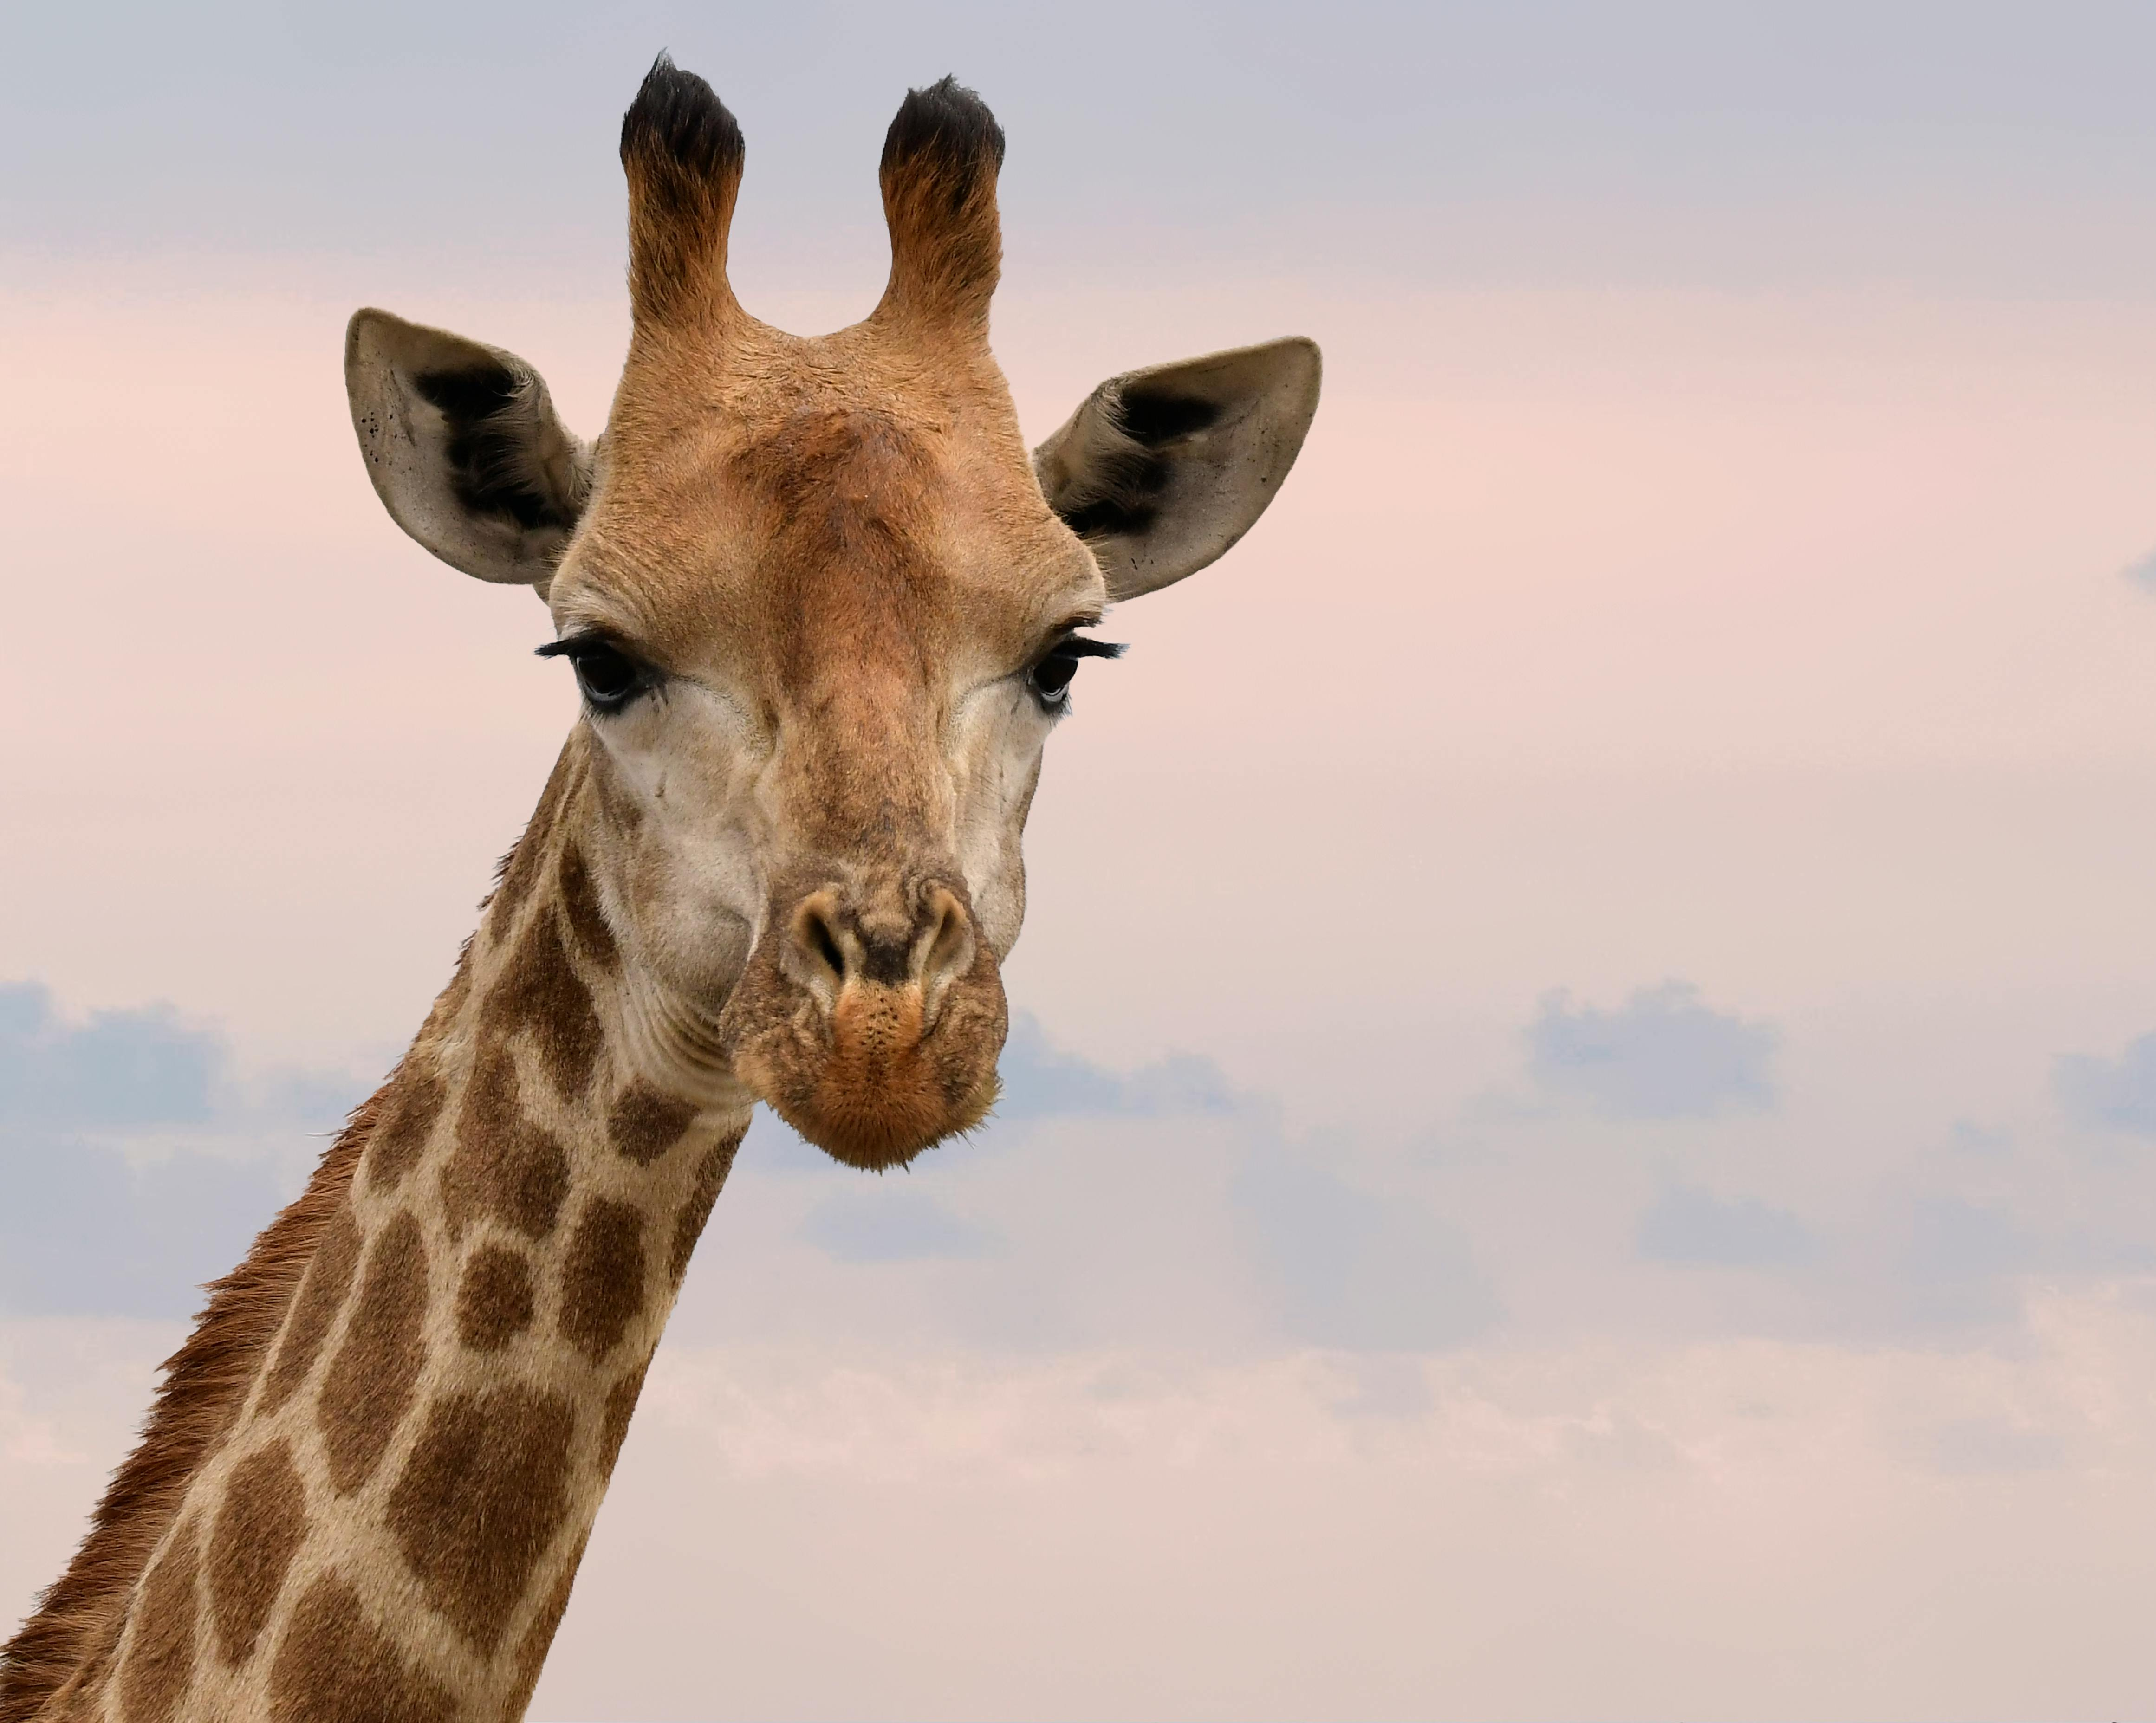
\includegraphics[width=0.5\linewidth]{figures/paper_a/pexels-frans-van-heerden-201846-802112.jpg}
    \caption{Giraffe, Frans van Heerden: https://www.pexels.com/de-de/foto/nahaufnahme-fotografie-der-giraffe-802112/ }
    \label{m:fig:giraffe}
\end{figure}
\clearpage

\chapter{Chapter Two}
\label{cha:two}

Lorem ipsum dolor sit amet, consetetur sadipscing elitr, sed diam nonumy eirmod tempor invidunt ut labore et dolore magna aliquyam erat, sed diam voluptua. At vero eos et accusam et justo duo dolores et ea rebum. Stet clita kasd gubergren, no sea takimata sanctus est Lorem ipsum dolor sit amet. Lorem ipsum dolor sit amet, consetetur sadipscing elitr, sed diam nonumy eirmod tempor invidunt ut labore et dolore magna aliquyam erat, sed diam voluptua. At vero eos et accusam et justo duo dolores et ea rebum. Stet clita kasd gubergren, no sea takimata sanctus est Lorem ipsum dolor sit amet.


Therefore, this chapter presents research that structures existing research and conceptual knowledge to understand the function of \ac{bpm} (\Cref{sec:two_b}; \Citen{paper_b}). 


\section{Part One A}
\label{sec:two_b}

Lorem ipsum dolor sit amet, consetetur sadipscing elitr, sed diam nonumy eirmod tempor invidunt ut labore et dolore magna aliquyam erat, sed diam voluptua. At vero eos et accusam et justo duo dolores et ea rebum. Stet clita kasd gubergren, no sea takimata sanctus est Lorem ipsum dolor sit amet. Lorem ipsum dolor sit amet, consetetur sadipscing elitr, sed diam nonumy eirmod tempor invidunt ut labore et dolore magna aliquyam erat, sed diam voluptua. At vero eos et accusam et justo duo dolores et ea rebum. Stet clita kasd gubergren, no sea takimata sanctus est Lorem ipsum dolor sit amet.


\clearpage

\clearpage
\chapter{Conclusion}
\label{cha:Conclusion}

\section{Summary}
\label{sec:Summary}  

    
\section{Limitations and Outlook}
\label{sec:Limitations}


\paragraph*{Use of writing assistance}
Please note that I have utilized various writing assistance software programs (e.g., ChatGPT, DeepL, and Grammarly) to enhance the language and readability of this work. Nevertheless, I take full responsibility for its content and have thoroughly reviewed and edited the material as necessary.
\clearpage

%% Bibliography %%
\printbibliography[notcategory=ignore,heading=bibintoc]
\newpage

%% Appendix %%
\appendix

\chapter{Overview of Research Papers}
\label{cha:app}

\section{Research Papers Included in This Dissertation}
\label{sec:app_papers}

\paperEntry{paper_a}
(VHB-JQ3\footnote{VHB-JQ3: VHB-JOURQUAL3}: B, 
VHB-JQ4\footnote{VHB-JQ4: VHB Publication Media Rating 2024}: B,
ABDC\footnote{ABDC: Australian Business Deans Council Journal Quality List}: A, 
SJR\footnote{SJR: Scimago Journal \& Country Rank, 2023}: Q1, 
IF\footnote{IF: Impact Factor, 2023}: 7.4)

\paperEntry{paper_b}
% computers in industry
(VHB-JQ3: C, 
VHB-JQ4: B,
ABDC: -, 
SJR: Q1, 
IF: 8.2)



\section{Index of Further Papers}
\label{app:sec:further}

Over the course of the dissertation, I also authored and co-authored the following research papers, studies, and reports.
These papers are not part of this dissertation.

\fullcite{paper_xyz}


\section{Individual Contribution to the Included Research Papers}
\label{sec:contributions}
    

This cumulative dissertation comprises two research papers, all co-authored with multiple collaborators. 
This section details the context and outlines my contributions to the two papers. 
The descriptions adhere to the \ac{credit} \citep{allen_2019_HowCan}.

\paperContrib{paper_a} was written by a team of three authors. 

\paperContrib{paper_b} was written by a team of three authors. 


\clearpage

\longEntry{paper_a}{P1: Paper A -- title used in the PDF Navigation Section}

\longEntry{paper_b}{P2: Paper B -- for pdf navigation}

\end{document}
